% Options for packages loaded elsewhere
\PassOptionsToPackage{unicode}{hyperref}
\PassOptionsToPackage{hyphens}{url}
%
\documentclass[
  oneside]{book}
\usepackage{amsmath,amssymb}
\usepackage{lmodern}
\usepackage{ifxetex,ifluatex}
\ifnum 0\ifxetex 1\fi\ifluatex 1\fi=0 % if pdftex
  \usepackage[T1]{fontenc}
  \usepackage[utf8]{inputenc}
  \usepackage{textcomp} % provide euro and other symbols
\else % if luatex or xetex
  \usepackage{unicode-math}
  \defaultfontfeatures{Scale=MatchLowercase}
  \defaultfontfeatures[\rmfamily]{Ligatures=TeX,Scale=1}
\fi
% Use upquote if available, for straight quotes in verbatim environments
\IfFileExists{upquote.sty}{\usepackage{upquote}}{}
\IfFileExists{microtype.sty}{% use microtype if available
  \usepackage[]{microtype}
  \UseMicrotypeSet[protrusion]{basicmath} % disable protrusion for tt fonts
}{}
\makeatletter
\@ifundefined{KOMAClassName}{% if non-KOMA class
  \IfFileExists{parskip.sty}{%
    \usepackage{parskip}
  }{% else
    \setlength{\parindent}{0pt}
    \setlength{\parskip}{6pt plus 2pt minus 1pt}}
}{% if KOMA class
  \KOMAoptions{parskip=half}}
\makeatother
\usepackage{xcolor}
\IfFileExists{xurl.sty}{\usepackage{xurl}}{} % add URL line breaks if available
\IfFileExists{bookmark.sty}{\usepackage{bookmark}}{\usepackage{hyperref}}
\hypersetup{
  pdftitle={化险为夷------与复杂性和波动性共舞的艺术},
  pdfauthor={广予},
  hidelinks,
  pdfcreator={LaTeX via pandoc}}
\urlstyle{same} % disable monospaced font for URLs
\usepackage{longtable,booktabs,array}
\usepackage{calc} % for calculating minipage widths
% Correct order of tables after \paragraph or \subparagraph
\usepackage{etoolbox}
\makeatletter
\patchcmd\longtable{\par}{\if@noskipsec\mbox{}\fi\par}{}{}
\makeatother
% Allow footnotes in longtable head/foot
\IfFileExists{footnotehyper.sty}{\usepackage{footnotehyper}}{\usepackage{footnote}}
\makesavenoteenv{longtable}
\usepackage{graphicx}
\makeatletter
\def\maxwidth{\ifdim\Gin@nat@width>\linewidth\linewidth\else\Gin@nat@width\fi}
\def\maxheight{\ifdim\Gin@nat@height>\textheight\textheight\else\Gin@nat@height\fi}
\makeatother
% Scale images if necessary, so that they will not overflow the page
% margins by default, and it is still possible to overwrite the defaults
% using explicit options in \includegraphics[width, height, ...]{}
\setkeys{Gin}{width=\maxwidth,height=\maxheight,keepaspectratio}
% Set default figure placement to htbp
\makeatletter
\def\fps@figure{htbp}
\makeatother
\setlength{\emergencystretch}{3em} % prevent overfull lines
\providecommand{\tightlist}{%
  \setlength{\itemsep}{0pt}\setlength{\parskip}{0pt}}
\setcounter{secnumdepth}{5}
\usepackage{ctex}

%\usepackage{xltxtra} % XeLaTeX的一些额外符号
% 设置中文字体
%\setCJKmainfont[BoldFont={黑体},ItalicFont={楷体}]{新宋体}

% 设置边距
\usepackage{geometry}
\geometry{%
  left=2.0cm, right=2.0cm, top=3.5cm, bottom=2.5cm} 

\usepackage{amsthm,mathrsfs}
\usepackage{booktabs}
\usepackage{longtable}
\makeatletter
\def\thm@space@setup{%
  \thm@preskip=8pt plus 2pt minus 4pt
  \thm@postskip=\thm@preskip
}
\makeatother
\ifluatex
  \usepackage{selnolig}  % disable illegal ligatures
\fi
\usepackage[style=apa,]{biblatex}
\addbibresource{mybib.bib}

\title{化险为夷------与复杂性和波动性共舞的艺术}
\author{广予}
\date{2022年11月26日}

\begin{document}
\maketitle

{
\setcounter{tocdepth}{1}
\tableofcontents
}
\hypertarget{ux524dux8a00}{%
\chapter*{前言}\label{ux524dux8a00}}
\addcontentsline{toc}{chapter}{前言}

这是一本关于保险历史、金融和科技的书。它将通过开源协作的方式不断更新。它将秉承尽早出版,经常出版(Publish Early and
Publish Often)的理念,立志于解决两个问题:

\begin{itemize}
\tightlist
\item
  作为一个建造者(Builder),如何设计一个足够灵活的系统抵抗自然的无常风险,甚至不断壮大?
\item
  作为一个交易者(Trader),如何在肥尾分布的世界对冲、套利、投资获益?
\end{itemize}

这本书受到了查理芒格思维栅格的影响,希望用跨学科方式去给出最基础的模型并在现实世界中反复交叉运用。
目前探讨的主题包括但不限于:心理学(时间偏见、心理会计)、精算概率、认识论(东西方差异)、编程实践(增量开发与星云假说隐喻)
中国哲学(道家、管子轻重学)、人体医学与复杂的层级。

\hypertarget{ux591cux5954ux5927ux540cux98ceux9669ux8f6cux79fbux4e0eux5747ux644aux7684ux5927ux524dux63d0}{%
\chapter{夜奔大同------风险转移与均摊的大前提}\label{ux591cux5954ux5927ux540cux98ceux9669ux8f6cux79fbux4e0eux5747ux644aux7684ux5927ux524dux63d0}}

遍地狼烟的时代,少年侠客夜奔山西大同,投靠了镖局。以晋商为依托,他们的业务线南则佛山,东则苏州,西至汉口,北达京师。
镖局,或许是中国古代最早的保险公司的雏形。

如果你是少年侠客,那就必须从预设的大前提出发,否则便会沦为经验与数据的囚徒,被官场、商场、江湖所纷扰,一无所获。

想称雄百年,有三个前提帮助你做演绎推理:

\begin{enumerate}
\def\labelenumi{\arabic{enumi}.}
\item
  保险投资活动是时间的长河中源源不断刷新的随机过程,它不是某一段时间内的一次性投资,
  也不是某一段时间内多次投资运输任务的算术加总。
\item
  保险游戏的目标不是最大化理论家构想出来的某个期望值,也不是打败我们随意选取的某个评估基准(Artifical Benchmark),
  而是在时间的河流中优化复合年化增长率与落袋为安的最终财富(Realized Ending Wealth)。
  这个游戏的目的不是单次的赢或者输,而是边界本身的不断扩张。这个游戏玩的是规则本身。
\item
  永远从反面出发,最优化复合年化增长率等价于最小化年化负面波动税率。
  如果某项策略能够以足够便宜的价格降低风险,那就该考虑把这项策略加入投资组合,以增加在时间长河中的复合年化增长率。
\end{enumerate}

\hypertarget{ux91cfux624dux80dcux5df1ux4fddux9669ux79d1ux6280ux7684ux56e2ux961fux6587ux5316ux5efaux8bbe}{%
\chapter{量才胜己------保险科技的团队文化建设}\label{ux91cfux624dux80dcux5df1ux4fddux9669ux79d1ux6280ux7684ux56e2ux961fux6587ux5316ux5efaux8bbe}}

将者,智、信、仁、勇、严也。

好的品德是穿越大时间周期自然选择的生存策略。团队里的新手才能一开始有所欠缺,良好的品德会让他的成长迅速。
如果你发现一个团队中充斥了以下这些文化觅母,战斗力起码不会弱。

比如,谦虚。谦虚的工程师深知大型项目的复杂度以及自己的局限。所以他会

\begin{itemize}
\tightlist
\item
  主动谋求队友的批评与检查
\item
  缩短反馈回路
\item
  遵循已经被证明的最佳实践
\item
  面向问题而不是执行细节编程。
\end{itemize}

比如,诚实。诚实的队友在犯错的第一时间会承认错误,及时止损并且内省。他会提供解决方案;丰富自己的经验;思考如何从错误中获利。
相反,不诚实的队友会和你说这一切都是天气不好或者老板的某个阴谋。知错能改,善莫大焉。

比如,好奇。在日新月异的应用人工智能领域,好奇的队友拒绝自我重复,他会感到深深的不满。
如果他感到自己一直在做紧急而不重要的事,只在做行为改变而不是结构调整,他会抗议。他的好奇会促使他:

\begin{itemize}
\tightlist
\item
  动手做实验。发现最适合当下自己的开发模式。
\item
  阅读如何解决问题和认知科学相关的元知识。
\item
  他始终好奇同样的任务有没有更好的解决方案。
\end{itemize}

比如,纪律。纪律非但是降低错误率的手段,也是创造力的来源。乔布斯说过,创新是对一千件事情说不,只有纪律和给自己约束,精力才能在重大的创新上燃烧。
知止而后能定。为自己的工作制定纪律,比如:测试驱动开发、重构、写短小的模块化的函数、用简单的设计,似乎是给自己上了枷锁,但其实打开了创造力的大门。

比如,乐于合作。己所不欲勿施于人,他不会直接把一团乱麻的代码交给同事去修改。对一个优秀工程师而言,代码是写给人看的,接着才是机器执行的。
对自己踩过的坑,他会及时把解决方案写在公共文档里。

\hypertarget{ux4e3aux4ec0ux4e48ux8bfaux5956ux5f97ux4e3bux4e0dux7528ux81eaux5df1ux7684ux5f97ux5956ux7b56ux7565ux6295ux8d44}{%
\chapter{为什么诺奖得主不用自己的得奖策略投资?}\label{ux4e3aux4ec0ux4e48ux8bfaux5956ux5f97ux4e3bux4e0dux7528ux81eaux5df1ux7684ux5f97ux5956ux7b56ux7565ux6295ux8d44}}

1952年,哈里马克维茨(Harry Markowitz)的发表了成名作``投资组合选择''。四十年后,他的均值方差模型拿到了诺奖。
但令人玩味的是哈里马克维茨自己在接受媒体采访时,却说他不用自己的策略投资,而是用一种更简单的策略:把自己的钱均匀分配到
他看好的N个基金中。

万物皆权衡,现代投资组合理论(Modern Portfolio Theory)指导下的分散化投资其实就是以杠杆风险的增高(依赖模型参数的准确性)换取了集中性风险的降低。
如果死扣理论,我们需要根据少有的历史数据对大量的参数------一个协方差矩阵的元素------进行估计。稍有不慎再加上一些盲目乐观的杠杆,就能炸毁整个金融系统,参见
1998年的长期资本管理公司(LTCM)事件。历史讽刺地让这个取名为``长期''的公司在短期内就破产了。

\hypertarget{ux6df7ux6dc6ux98ceux9669ux6a21ux578bux4e0eux6a21ux578bux98ceux9669}{%
\section{混淆风险模型与模型风险}\label{ux6df7ux6dc6ux98ceux9669ux6a21ux578bux4e0eux6a21ux578bux98ceux9669}}

人们非常容易混淆风险模型与模型风险两个截然不同的观念。大模型当道,有限的注意力转向了模型揭示的近期、显性的风险,从而忽略了远期的过分依赖模型带来的风险。
模型风险不是指奢望发现未来不可预测的事,历史就是不可预测而跳变的。模型风险是指可预测的逻辑上必然发生的事,但是由于我们过度依赖模型,我们认为它们离发生还很远。

师法自然,用模型进攻而不是防守。用模型产生数据而不是分析数据。防守主要是靠冗余。
当系统中建筑进一定的冗余度而非过分天真优化时,才能不被空头挤压(short squeeze)。

\hypertarget{ux53cdux5411ux5965ux5361ux59c6ux5243ux5200ux539fux5219}{%
\section{反向奥卡姆剃刀原则}\label{ux53cdux5411ux5965ux5361ux59c6ux5243ux5200ux539fux5219}}

在实践而不是理论领域,或许我们应该遵循反向奥卡姆剃刀原则。
在理论中,多个竞争模型如果都能解释和预测数据,我们选择最简单的那个。
但是在实践中,尤其是风险管理生意如保险或期权,多种策略如果都能达到目标,我们选冗余最多的那个。
天知道,一觉醒来,明天又会发生什么。

在实践中,如果经验与模型不一致时,左派书呆子会强行扭曲经验来适应模型。右派业务员可能会扭曲模型来适应经验。
其实两者可能都出错了,模型也错了,经验也错了。这时候需要重新更新行为和认知框架。

\hypertarget{ux53c2ux8003ux6587ux732eux4e0eux6838ux5fc3ux6982ux5ff5}{%
\section{参考文献与核心概念}\label{ux53c2ux8003ux6587ux732eux4e0eux6838ux5fc3ux6982ux5ff5}}

\begin{enumerate}
\def\labelenumi{\arabic{enumi}.}
\tightlist
\item
  奥卡姆剃刀原则(Occam's razor)、现代投资组合理论
\item
  Bowell(2011). Simple heresy: Rules of thumb challenge complex financial analyses.
\end{enumerate}

\hypertarget{ux53cdux5411ux4fddux9669ux516cux53f8ux4e0eux5723ux5f7cux5f97ux5821ux6096ux8bba}{%
\chapter{反向保险公司与圣彼得堡悖论}\label{ux53cdux5411ux4fddux9669ux516cux53f8ux4e0eux5723ux5f7cux5f97ux5821ux6096ux8bba}}

故事要从1713年的巴塞尔说起,尼古拉斯·伯努利(Nikolaus Bernoulli)问你假如抛一次硬币朝上,你赢2块钱,如果反面,继续游戏,第二次硬币朝上,你赢4块钱,如果反面,继续游戏,以此类推,第n次硬币朝上,你赢2的n次方块钱。请问你愿意出多少钱参加这个游戏?

这个问题的悖论之处在于即使你知道它的期望是正无穷,你也不会花很多钱参加这个游戏。

如果我们进一步简化这个问题,把它改成更简洁的掷筛子问题:
如果筛子为1,你赢1块钱,如果筛子为2,你赢2块钱,
如果筛子为3,你赢6块钱,如果筛子为4,你赢22块钱,
如果筛子为5,你赢200块钱,如果筛子为6,你赢1,000,000块钱。
请问你愿意出多少钱参加这个游戏?

显然你不会出500,000块去博1,000,000块的奖金,因为你知道很有可能你会扔到1,输掉499,999的钱。

1738年,丹尼尔伯努利(Daniel Bernoulli)提出了解决这个悖论的三个核心洞见:

\begin{itemize}
\tightlist
\item
  每个人的资源都是有限的,他的本金与风险承受能力是有限的。
\item
  金钱带给人的边际效用递减。这里他提出了核心概念边际效用。
\item
  人们不能买未来还没被卖的机会。时间概率与集合概率之间有区别。
\end{itemize}

假设你有100,000元的本金,我们可以模拟各种付出的数量,并且计算六种情况下游戏结束以后你最终财富的几何平均期望。
假设你花50,000参与游戏为例,最终的几何期望收益就是(50001\emph{50002}50006\emph{50022}50200*10050000) ** 1/6 =56624元远远低于你原来的100,000元。

这个版本的圣彼得保悖论告诉我们如果从几何期望而不是算术期望的角度来看待问题,我们就能解开这个悖论。

下面我们在来思考圣彼得堡悖论的另一个版本,这与保险公司的生意有关。

假设你是一个大航海时代的船长,你有本金3000元,如果跑成一单货你会获得13000元的收入,净赚10000元。
但是大海上海盗林立,强匪横行,你的船有5\%的概率被劫持,这会导致你承受10000元的损失。你在考虑要不要买保险?
保险公司给你开出的条件是,你交800元的保费,如果你的船被劫持,保险公司会给你赔偿10000元。

你算了一下觉得保险公司太黑心,为数学期望站在了它们一边:
-800 * 0.95 + (10000 - 800) * 0.05 = -300

或许你的内心还会嘀咕,这完全就是一个兜售恐惧的生意。

但是如果你从几何期望的角度来看待问题,你会发现购买了这个合同,在这个案例中,你与保险公司达成了正和博弈而非零和博弈。

如果不买保险,站在你的角度几何期望的计算就变成了:
((13000\^{}95) * (3000\textsuperscript{5))}1/100)= 12081元

如果你买了保险,你的最差收益就是13000-800 = 122000元。从几何期望的角度考虑,你收益了119元。

如果你是希望长期在这个运输行业立足,进行多轮博弈,你的目标是最大化你的年化增长率(compound annual growth rate)
而不是某个臆想出来的数学期望(mathematical expectation)。在这种情况下,在你的组合中加入保险公司的保险合同,是一个
成本有效(cost effective)的选择。

我们跳出航海时代,回到1955年的现实世界,那一年克拉默提出了保险生意的两个基本问题:

\begin{itemize}
\tightlist
\item
  如何计算保险公司破产的概率?
\item
  如何刻画理赔总量的分布?
  他写下了以下公式来描述:
  U(t) = U + c(t) - S(t)
  其中,U是公司的初始本金(initial capital),c(t)代表保费收入率,S(t)是保单到达的过程。
\end{itemize}

从这个公式出发,我们可以得到两种不同的赚钱策略:
第一种策略是几乎每次都能赚钱,赚取稳定的保费,并确保黑天鹅事件带来的损失不会超过之前保费的总收入。

第二种策略更像是反向保险公司策略,它反其道而行之,它通过高频的小额的局部的损失来换取巨大的收益。这种策略被以塔勒布、马克·斯匹兹纳戈等人发挥地炉火纯青。
他们称自己为危机狩猎者(Crisis hunter)。

第一种策略更像是赌场盈利的策略,第二种是赌徒利用赌场对小概率时间带来的影响系统性低估而盈利的策略,它们互为其根。

第二种策略要求人在心理上不断地经历``将欲取之必先予之''的过程,有很强的反直觉性,本文所做的工作就是直追它诞生的历史冒险源头和思想源头
1713年的圣彼得堡悖论与波澜壮阔但是残酷血腥的大航海时代。

\hypertarget{ux4e0dux53efux80dcux5728ux5df1ux7684ux7f16ux7801ux4e0eux4ea4ux6613ux98ceux9669ux7ba1ux7406}{%
\chapter{不可胜在己的编码与交易风险管理}\label{ux4e0dux53efux80dcux5728ux5df1ux7684ux7f16ux7801ux4e0eux4ea4ux6613ux98ceux9669ux7ba1ux7406}}

孙子曰:善战者,先为不可胜,以待敌之可胜。不可胜在己,可胜在敌。同样,1903年瑞士精算学家Flip Lundberg提出了``毁灭问题''。在考虑如何盈利前,我们应该先考虑破产的风险。破产问题是指,假设你有一笔初始本金,客户的索赔率以服从泊松过程的强度到达,
你收一个常熟项的保费(preimum rate),如何计算你开的公司破产的概率?

带着这个思维框架,去重新思考编码与交易,我们获得一种新的角度:
给定一笔本金,假设市场上每个到期的合约以服从某个过程的强度到达,我们如何计算交易破产的概率?
给定一个交付日期,假设不停变化的要求以服从某个过程的强度到达,我们如何计算项目无法交付的概率?

在这种角度下,我们不在关注市场与客户需求的变化怎样影响我们的盈利,而是关注我们对持续变化的反应是怎样影响我们的盈利。如果没有风险管理协议的设计与执行,从长期来看(甚至不用多长几天和几周就能看出来),自己爆炸和破产都是注定的事。

\hypertarget{ux4ea4ux6613ux98ceux9669ux7ba1ux7406}{%
\section{交易风险管理}\label{ux4ea4ux6613ux98ceux9669ux7ba1ux7406}}

交易风险管理可以从交易前,交易中和交易后三个角度考虑。每笔交易,都是迈入一场残酷的战争,
在迈入战争前,我们需要问自己以下四个问题:

\begin{itemize}
\tightlist
\item
  我的风险/收益比、几何期望收益与目标盈利是多少?
\item
  我能承受的最大损失是多少?
\item
  我即将开始的交易是为了赚钱还是为了管理风险,还是牺牲其中一个来换取另一个?
\end{itemize}

在交易中,我们需要问自己以下三个问题:

\begin{itemize}
\tightlist
\item
  交易是否达到了我们之前制定的最大损失?
\item
  交易是否达到了我们之前制定的目标盈利?
\item
  我们是否值得冒险,让交易继续下去?
\end{itemize}

在交易后,我们需要复盘,问自己以下两个问题:

\begin{itemize}
\tightlist
\item
  我自己是否遵守了风险管理协议?
\item
  如果没有,我为什么没有遵守?
\end{itemize}

兵法:一曰度,二曰量,三曰数,四曰称,五曰胜。在资源管理上,头寸管理与强行止损也是需要养成的肌肉记忆。在每笔交易中,不要冒超过2\%的风险,如果在某两周或者一个月内,你的账户亏损超过6\%,那么就停止交易,直到下一个月。这会防止你的两种死法:

\begin{enumerate}
\def\labelenumi{\arabic{enumi}.}
\tightlist
\item
  犯系统性的错误而不自知,不停地流血,一错再错,进入死亡循环。
\item
  某一单出现巨额亏损,直接爆炸。
\end{enumerate}

\hypertarget{ux7f16ux7801ux98ceux9669ux7ba1ux7406}{%
\section{编码风险管理}\label{ux7f16ux7801ux98ceux9669ux7ba1ux7406}}

如果把每一次的编程都当成是我们碳基大脑与硅基大脑的交易,那我们也可以将风险管理的原则与编程手艺的最佳实践结合起来。

下表展示了风险管理策略与测试驱动开发原则的对应关系:

\begin{longtable}[]{@{}
  >{\raggedright\arraybackslash}p{(\columnwidth - 4\tabcolsep) * \real{0.33}}
  >{\raggedright\arraybackslash}p{(\columnwidth - 4\tabcolsep) * \real{0.33}}
  >{\raggedright\arraybackslash}p{(\columnwidth - 4\tabcolsep) * \real{0.33}}@{}}
\toprule
风险管理策略 & 实例 & 测试驱动开发原则 \\
\midrule
\endhead
分摊 & 两次下注\$5000,而不是一次下注\$10000 & 从测试------编码------重构三个正交的维度去解决一个问题而不是从一个维度去解决一个问题 \\
多样化 & 两个人各下注\$5000,而不是一个人下注\$10000 & 单元测试需要正交且互相独立,最大程度上减少依赖 \\
止损 & 不要冒超过2\%的风险,如果在某两周或者一个月内,你的账户亏损超过6\%,那么就停止交 & 一旦测试出错,就删去对应的生产代码,大脑退回到上一个状态中重新思考 \\
\bottomrule
\end{longtable}

如果没有测试驱动开发,你就很难重构以及持续集成和持续交付。在交易中,你每晚都会平仓,因为你不想冒你无法管理的风险。
在编码中,你希望所有的编码改变都能客户具体的反馈。

\hypertarget{ux63a8ux8350ux4e66ux76eeux4e0eux6838ux5fc3ux6982ux5ff5}{%
\section{推荐书目与核心概念}\label{ux63a8ux8350ux4e66ux76eeux4e0eux6838ux5fc3ux6982ux5ff5}}

\begin{enumerate}
\def\labelenumi{\arabic{enumi}.}
\tightlist
\item
  破产问题、风险管理、测试驱动开发
\item
  Mandelbrot, Benoit, and Richard L. Hudson. The Misbehavior of Markets: A fractal view of financial turbulence. Basic books, 2007.
\item
  Beck, K. (2003). Test-driven development: by example. Addison-Wesley Professional.
\item
  Martin, R. C. (2011). The clean coder: a code of conduct for professional programmers. Pearson Education.
\item
  孙武, \& 郭化若. (1900). 孙子兵法--. BEIJING BOOK CO. INC..
\end{enumerate}

\hypertarget{ux7978ux516eux798fux6240ux501aux9519ux4e86ux5224ux65adux4f46ux8d62ux4e86ux5e02ux573a}{%
\chapter{祸兮福所倚------错了判断,但赢了市场}\label{ux7978ux516eux798fux6240ux501aux9519ux4e86ux5224ux65adux4f46ux8d62ux4e86ux5e02ux573a}}

如果把每一笔交易都当成一场战争,那么在投入到血雨腥风之前,
我们必须先算好自己的获胜概率与下注的金额(dosage or betting ratio),否则就容易赢了概率输了赌局。
但如果我们的下注比例调整准确则可以如爱德华.索普(Edward Thorp)说的那样用庄家的钱赚钱。
曹操批孙子兵法有云:``故战必先算其费,因粮于敌也。''
1992年,爱德华.索普与Louis Rotando联合发表了凯利判据(Kelly Criterion)是如何应用于股票市场的资源分配问题的。

\hypertarget{ux51efux5229ux5224ux636eux7684ux6838ux5fc3ux601dux60f3}{%
\subsection{凯利判据的核心思想}\label{ux51efux5229ux5224ux636eux7684ux6838ux5fc3ux601dux60f3}}

假设你有一笔初始资金,你和庄家对赌,庄家拥有远大于你的接近无限的本金,但是设你用演绎法获得了一些信息优势。
每次赌局,你获胜的概率是0.7,而庄家获胜的概率是0.3。现在问你每笔赌局你应该下注多少,才能最大化你的收益,同时避免赌徒毁灭的困局。

爱德华.索普创造性地调整了优化的指标,既不是最小化毁灭的概率E(x0-\textgreater0),而不是最大化收益E(xn),而是最大化资本增长率对数转化下的几何平均
而非算术平均即E(log(xn/x0)\^{}1/n)。如果我们要使得该值最大,那么每次下注的比例就是b - q/p,其中b是你潜在的获利除以你需要付出的成本,
p是你获胜的概率,q是你输的概率。

\hypertarget{ux51efux5229ux5224ux636eux4e0eux7b49ux52a0ux901fux8fd0ux52a8ux548cux4fe1ux606fux8bbaux7c7bux6bd4}{%
\subsection{凯利判据与等加速运动和信息论类比}\label{ux51efux5229ux5224ux636eux4e0eux7b49ux52a0ux901fux8fd0ux52a8ux548cux4fe1ux606fux8bbaux7c7bux6bd4}}

如果从信息论的视角去观察凯利希望最优化的增长率指数公式我们会发现它与香农信息熵公式的构造有惊人的相似。
香农信息熵公式为H(x) = -∑p(x)log(p(x))。香农信息熵提出的背景是在一个数据通信系统中,
假如我们有信息源,有通信渠道和接受者,如果一个系统完全没有背景噪音,那么信号可能丢失或损失,假如噪音太大
信号的传导不是最优的,所以我们需要找到一个合适的平衡点。

如果从物理运动视角去观察凯利判据,我们以下注的比例f为x轴,G(f)对数几何平均增长率为y轴,
我们会发现它与物理等加速运动的轨迹有惊人的相似。一旦下注比例超过了最优值,dy/dt速度就会变成负数。

\hypertarget{ux51efux5229ux5224ux636e-vs-ux73b0ux4ee3ux6295ux8d44ux7ec4ux5408ux7406ux8bba}{%
\subsection{凯利判据 vs 现代投资组合理论}\label{ux51efux5229ux5224ux636e-vs-ux73b0ux4ee3ux6295ux8d44ux7ec4ux5408ux7406ux8bba}}

现代投资理论假设资产的收益率服从正态分布,并且对基于历史数据的协方差矩阵的参数估计准确性要求很高。
它假设你对所有资产的联合概率分布有一个很好的估计,但是在实际中,我们很难得到这样的估计。相反,如果我们
在实践中使用凯利判据,我们要做的是不断根据最坏情况和期望收益的比例动态调整我们的下注比例,在投资组合的配比领域,
凯利判据相比于现代投资组合理论或许有更好的抗模型风险能力。如我们在第二篇文章讨论的,模型风险与风险模型
是两个截然不同但是容易混淆的概念。

\hypertarget{ux63a8ux8350ux4e66ux76eeux4e0eux6838ux5fc3ux6982ux5ff5-1}{%
\section{推荐书目与核心概念}\label{ux63a8ux8350ux4e66ux76eeux4e0eux6838ux5fc3ux6982ux5ff5-1}}

\begin{enumerate}
\def\labelenumi{\arabic{enumi}.}
\tightlist
\item
  Thorp, E. O. (2008). The Kelly criterion in blackjack sports betting, and the stock market. In Handbook of asset and liability management (pp.~385-428). North-Holland.
\item
  Shannon, C. E. (1948). A mathematical theory of communication. The Bell system technical journal, 27(3), 379-423.
\end{enumerate}

\hypertarget{ux9047ux89c1ux4e94ux5341ux5e74ux540eux7684ux81eaux5df1}{%
\chapter{遇见五十年后的自己}\label{ux9047ux89c1ux4e94ux5341ux5e74ux540eux7684ux81eaux5df1}}

昔我往矣,杨柳依依。今我来思,雨雪霏霏。一个保险交易员有其独特于大众的时间偏好,
这种偏好称之为跨期交易偏好,他在过往与未来中穿梭,消解心中即时满足的渴,换之以绵密恒长的幸福心流。

我们因为生物之本能赋予当下的满足以极大的权重,在知觉上,在记忆中。
会计学和心理学的交叉领域中有个重要的概念叫``延迟折扣或者双曲线折扣(Hyperbolic Discounting)'',
它是指在有限的时间压力下,人们相比起未来的奖励给予当下的即时的奖励更高的优先级。
人类在进化中形成的双曲线折扣模型是一种变加速模型,遥远未来的贴现率在一开始的一小段以极大的加速度
衰减,越到后来加速度越小。相比而言,自然界中森林与鱼塘资源的衰减速度则更符合指数折扣模型(Exponential
Discounting)。

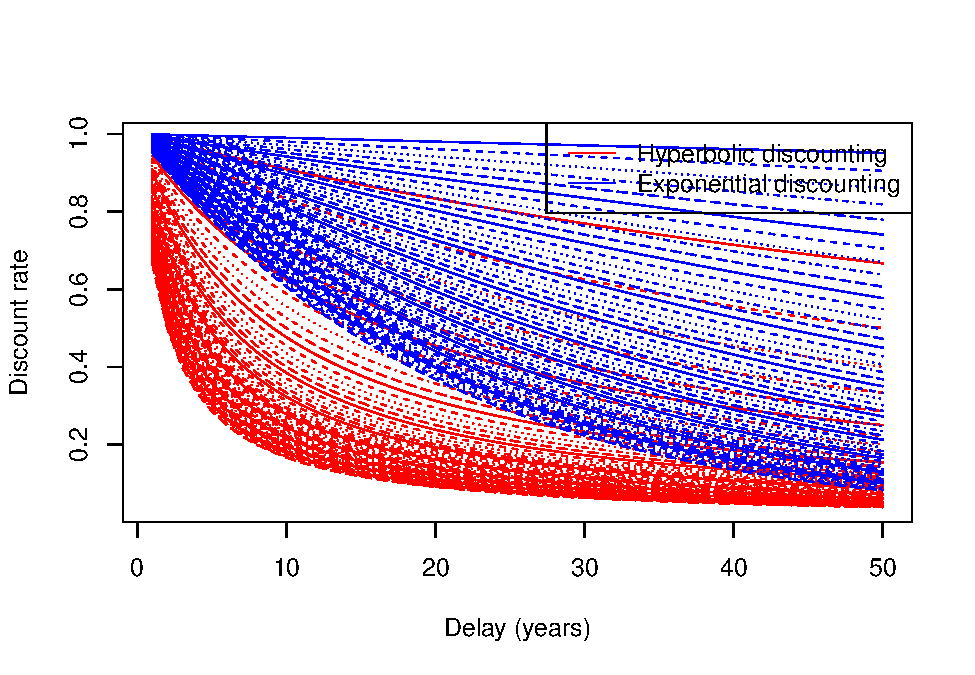
\includegraphics{6006-chapter06_files/figure-latex/unnamed-chunk-1-1.pdf}

任何非线性衍生品,都与时间相关。时间尤其是金融市场中的时间如流水,时而平缓,时而湍急。
它绝不是匀速运动,而是变加速运动,拥有极强的非线性特征。上世纪五十年代,某位MIT的名教授曾经天真地把自己根据开市价和收市价构建的数学模型进行交易,
他为自己制定的策略是:凡是市场上涨5\%或更多,购买并且持有。下跌5\%,抛售。回测结果显示他能大赚一笔但最后差点赔得倾家荡产。
该策略失败的主要原因是他忽略了日内价格的波动,这导致他想的是在上涨5\%的时候买,但是市场上一下子跳到了7.5\%,而想在下跌到5\%卖出时,
市场根本不给他机会,直接跌超了5\%。

如果我们承认自己对时间的觉知还留存着强烈的如动物般的及时满足的生物本能并且市场本身的时间运动规律与这种动物性不一致时,
那么如果能战胜自己让自己拥有独特的跨期时间偏好,比常人更加克制现在就要的冲动,便拥有了独特的优势。所谓胜人者有力,自胜者强。

知易行难。灵长类人科这一属出现距今约200万年,但是距今1万年左右,人类才开始了植物生产和人口数量的急剧增加。
司管理性推理和延迟满足的模块建成相比其他模块的时间可能只占到了1\%。在相同问题上,进化时间较近的模块与
久远的和本能生存相关的模块会有截然不同的决策结果。如果用意志力强行说服自己必然失败,我们需要和自己的原始大脑玩一些心理游戏
来帮助他曾经在进化中资源极度稀缺环境下必不可少但是在当下已经过时的策略。

\hypertarget{ux770bux4e00ux770bux8001ux53bbux7684ux81eaux5df1}{%
\subsection{看一看老去的自己}\label{ux770bux4e00ux770bux8001ux53bbux7684ux81eaux5df1}}

跨期交易的决策难做是因为我们的情绪和身体感受对当下的环境和即时的回报非常强烈,但是对于未来时间段的自己
很难感同身受。心理学家Hal Hershfield和Daniel Goldstein于是画出了老年时你可能变成的样子,
他们发现当你真实看到自己的白发与皱纹时,你更愿意储蓄与为未来的不确定性囤积资源,构建冗余而不是提前消费。
佛法里也有白骨观的修炼方法,看到死去的自己,腐烂的自己,来帮助人们守戒,得定,开慧。

\hypertarget{ux6267ux884cux610fux56fe}{%
\subsection{执行意图}\label{ux6267ux884cux610fux56fe}}

心理学家Peter Gollwitzer采取了新范式创新帮助人们从目标意图变成了执行意图。比如不让人制定我想要减肥或者
我想要减掉25公斤的目标,而是强迫人们思考与目标有关的情境。``明天睁眼以后(时间),我就要穿上床边的耐克鞋去校园(环境)旁边跑400米(行为)。''
``如果我心情感到愉悦时,我就会深蹲50磅。''它通过提前对行动的规划,降低你认知资源的消耗,加之高频率的重复成为一种生理本能。
你与未来的自己签一纸期权合约,把止损点、价格和回报时间都制定好,解耦了交易计划和交易执行的逻辑。自我的斗争变为了一种对未来自我慈爱的情绪。

\hypertarget{ux63a8ux8350ux4e66ux76eeux4e0eux6838ux5fc3ux6982ux5ff5-2}{%
\section{推荐书目与核心概念}\label{ux63a8ux8350ux4e66ux76eeux4e0eux6838ux5fc3ux6982ux5ff5-2}}

\begin{enumerate}
\def\labelenumi{\arabic{enumi}.}
\tightlist
\item
  Hershfield, H. E., Goldstein, D. G., Sharpe, W. F., Fox, J., Yeykelis, L., Carstensen, L. L., \& Bailenson, J. N. (2011). Increasing saving behavior through age-progressed renderings of the future self. Journal of marketing research, 48(SPL), S23-S37.
\end{enumerate}

\printbibliography

\end{document}
